\documentclass[main]{subfiles}
\begin{document}

\section{Current Correlator}
%Doris

\begin{figure}[htbp]
  \centering
  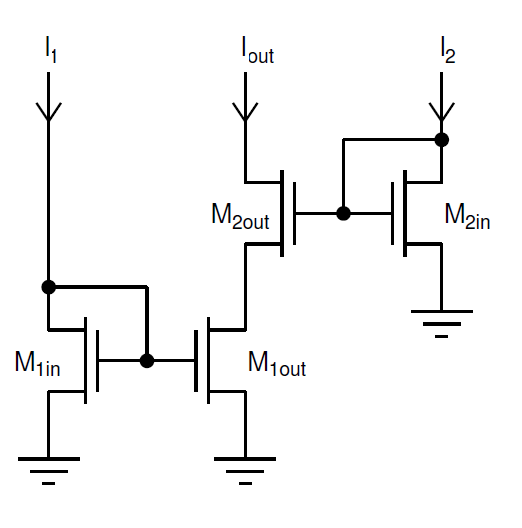
\includegraphics[scale=0.7]{pics/Current_correlator_circuit.png}
  \caption{Current correlator circuit}
  \label{fig:Current_correlator_circuit}
\end{figure}

The Current Correlator is comprised of two stacked current mirrors that have the output of one mirror ($M_2$) lead into the drain of the other mirror ($M_1$). Currents, $I_1$ and $I_2$, are sunk through the diode connected half of both mirrors, pulling $V_1$ and $V_2$, respectively, so that they follow: 

\begin{equation}
I_{out} = I_o e^{\kappa V_1}\cdot(1-e^{V}) \geq 0
\end{equation}


If $V_1 > V_2$, $M_1$ will sink $I_1$ and pull up the common node voltage V (of the $M_1$ drain voltage and $M_2$ source voltage), reducing the current through $M_2$. Thus $I_{out}$ settles at a self normalized product between $I_1$ and $I_2$. 

\begin{equation}
I_{out} = \frac{I_1 \cdot I_2}{I_1+I_2} \geq 0
\end{equation}

However, if $V_1$ is off, $I_2$ will charge common node V until $M_2$ shuts off once $V>V_{d_M2}+4U_t$. Likewise, if $M_2$ is off, the drain of $M_1$ will be off. 

\begin{figure}[htbp]
  \centering
  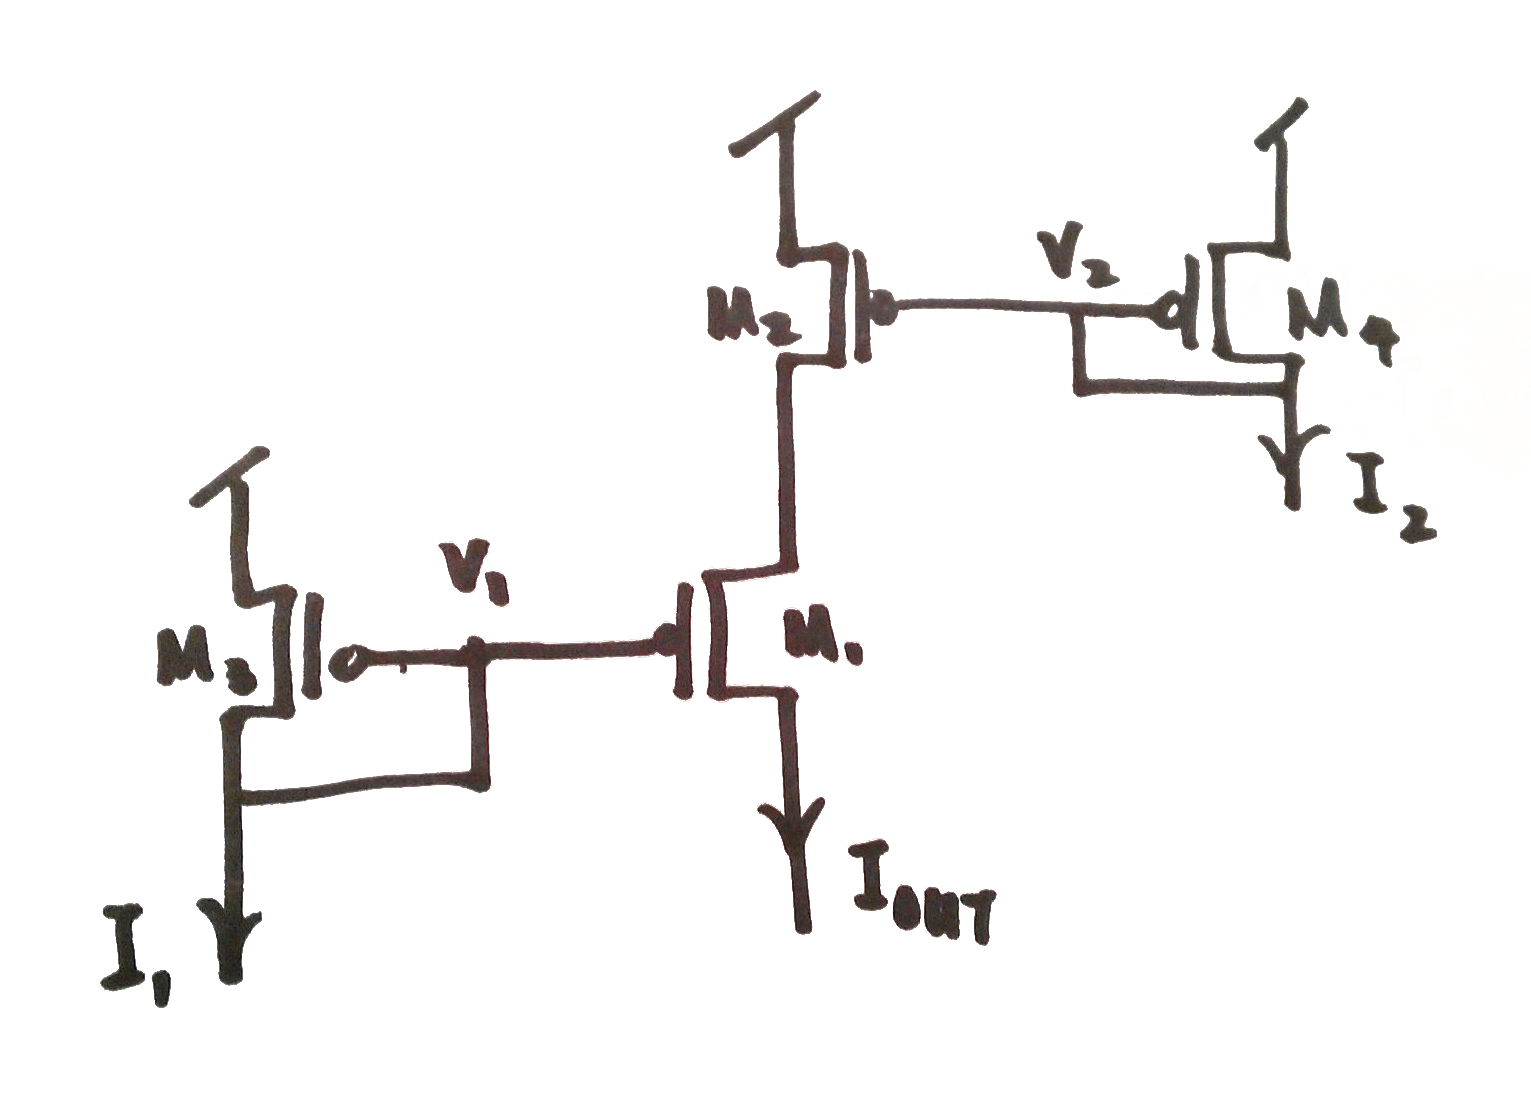
\includegraphics[scale=0.2]{pics/pFET_Current_correlator_circuit.png}
  \caption{pFET Current correlator$ \rightarrow$ two stacked pFET mirrors with 3 current sinks}
  \label{fig:pFET_Current_correlator_circuit}
\end{figure}
\end{document}